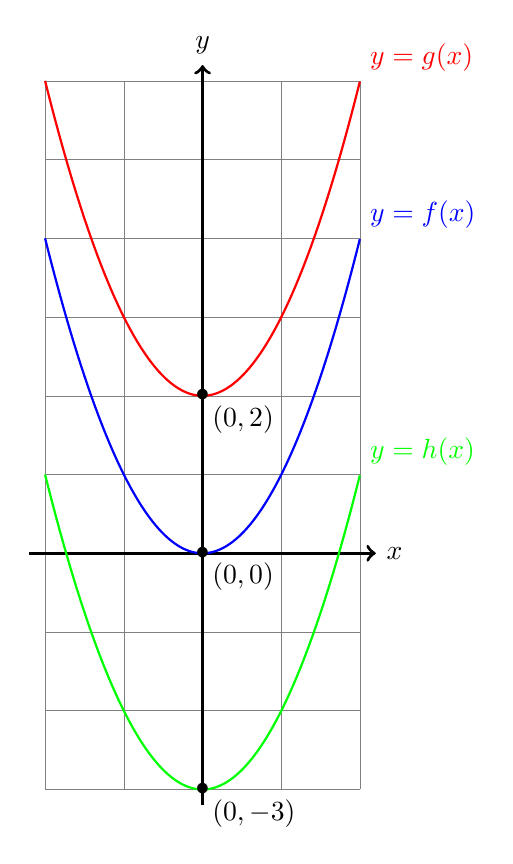
\begin{tikzpicture}[domain=-2:2]
  \draw[very thin,color=gray] (-2,-3) grid (2,6);

  \draw[very thick,->] (-2.2,0) -- (2.2,0) node[right] {$x$};
  \draw[very thick,->] (0,-3.2) -- (0,6.2) node[above] {$y$};
  
  \draw [color=blue,thick] plot[smooth,samples=500] (\x,{(\x)^2}) node [above right] {$y = f(x)$};
  \draw [color=red,thick] plot[smooth,samples=500] (\x,{(\x)^2 + 2}) node [above right] {$y = g(x)$};
  \draw [color=green,thick] plot[smooth,samples=500] (\x,{(\x)^2 - 3}) node [above right] {$y = h(x)$};

  \node at (0,0) {$\bullet$};
  \node [below right] at (0,0) {$(0,0)$};

  \node at (0,2) {$\bullet$};
  \node [below right] at (0,2) {$(0,2)$};

  \node at (0,-3) {$\bullet$};
  \node [below right] at (0,-3) {$(0,-3)$};
\end{tikzpicture}
